% TikZ plot for operational metrics
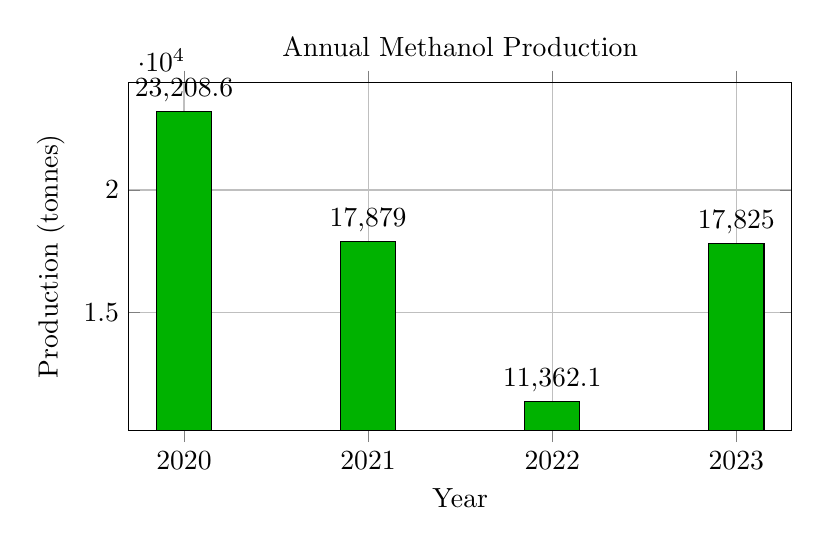
\begin{tikzpicture}
\begin{axis}[
    title={Annual Methanol Production},
    xlabel={Year},
    ylabel={Production (tonnes)},
    ybar,
    bar width=20pt,
    width=10cm,
    height=6cm,
    xtick=data,
    xticklabels={2020, 2021, 2022, 2023},
    nodes near coords,
    nodes near coords align={vertical},
    grid=major,
    legend pos=north west,
]

\addplot[fill=green!70!black,draw=black] coordinates {
    (2020, 23208.6)
    (2021, 17879.0)
    (2022, 11362.1)
    (2023, 17825.0)
};

\end{axis}
\end{tikzpicture}
